\documentclass[12pt]{article}
\usepackage[margin=1in]{geometry} 
% \usepackage[english]{babel}
\usepackage{amsmath}
\usepackage{tcolorbox}
\usepackage{amssymb}
\usepackage{amsthm}
\usepackage{lastpage}
\usepackage{fancyhdr}
\usepackage{accents}
\usepackage{hyperref}
\pagestyle{fancy}
\setlength{\headheight}{40pt}

\hypersetup{
    colorlinks=true,
    linkcolor=blue,
    filecolor=magenta,      
    urlcolor=cyan,
    pdftitle={Overleaf Example},
    pdfpagemode=FullScreen,
  }


\newenvironment{solution}
  {\renewcommand\qedsymbol{$\blacksquare$}
  \begin{proof}[Solution]}
  {\end{proof}}
\renewcommand\qedsymbol{$\blacksquare$}

\newcommand{\ubar}[1]{\underaccent{\bar}{#1}}

% \addbibresource{./resources/references.bib}

 % add packages, settings, and declarations in settings.tex

\title{Text Comprehension}
\author{Christian Bauer, 01560011}
\date{}

% \bibliographystyle{plain}
% \addbibresource{./resources/references.bib}

\begin{document}


\maketitle

% Report

% A report should be a 6-8 pages long document structured as a research paper, as shown below. You may modify this structure, but the suggested list is a good starting point.

\tableofcontents
    
\pagebreak

    \section{Motivation}
    \label{sec:motivation}

    % Motivation: describe the problem you are solving, explain why is it important, and provide a short summary of your methods and obtained results.

        % NLP is a hard task for computers and writing a chatbot that "understands" user input, meaning providing a satisfactory answer is a challenging task.
        % For the project, a chatbot will be implemented, which should be able to answer questions from the \emph{Stanford Question Answering Dataset} (short= \emph{SQuAD})\footnote{SQuAD source: \url{https://rajpurkar.github.io/SQuAD-explorer}}.
        % This dataset was extracted by volunteers with over 500 Wikipedia articles. 
        % Each of these articles is considered a title in the dataset and each holds numerous \emph{question-answer-sets (=QAS)}.
        % This SQuAD-dataset will be the source for the training dataset used to train the machine learning models.
        Natural Language Processing (NLP) is a hard task for computers and creating a system that is able to "comprehend" natural language to be able to provide a reasonable answer to questions is very challenging and a lot of research is done at the moment to improve NLP tasks.
        The first idea for this project was to implement a chatbot that will be build on top of a Feed Forward Neural Network (FNN).
        While researching resources for that task, a more interesting task was found, the comprehension of text with the help of deep learning.

        The task of natural language comprehension was a more challenging approach, since opposed to the chatbot using FNN that was used similar to a lookup table, finding the correct answer to a question given some context was a daring and unknown field to me.
        This comprehension is already widely used by companies such as Google, and often when you look for a topic, you get a well-defined short summary presented above all query objects.


    \section{Data}
    \label{sec:data}
    % Data: describe the data you are using in the project and provide examples. what kind of data you are using, where does it come from? what are the properties of your data, like balance, missing values, scale, etc., and what are you going to do about it? what kind of preprocessing, filtering, augmentation, or other manipulations are you applying in the project?  

        For the project, "The Stanford Question Answering Dataset (SQuAD)"\footnote{Source: https://rajpurkar.github.io/SQuAD-explorer/} will be used. This dataset was generated for reading comprehension training and the data is based on Wikipedia articles.
        There exist two versions of this dataset, \texttt{SQuAD 1.1} that holds 100,000 question-answer sets, and \texttt{SQuAD 2.0} that contains all question-answer sets from \texttt{SQuAD 1.1} and additionally also includes 50,000 question-answer sets that are unanswerable, and a modern reading comprehension system has to be able to also determine whether a question is answerable or not.


        \subsection{Example Data Element of SQuAD}
        \label{subsec:data-example}

            As an example, a section from the \texttt{Prime\_number} data chunk was taken as can be seen in figure \ref{fig:-squad-example}. On the left, the \emph{context} is shown, which is the text paragraph that contains the answer at some position.

            In the right column of the figure, the question is presented in bold letters, and the ground truth answer that is to be found is highlighted in green. \emph{Note: This is only partially represents the actual data that is provided by SQuAD.}


            \begin{figure}[h!]
                \centering
                \caption{SQuAD Example Question-Answer Set\cite{squadExample}}
                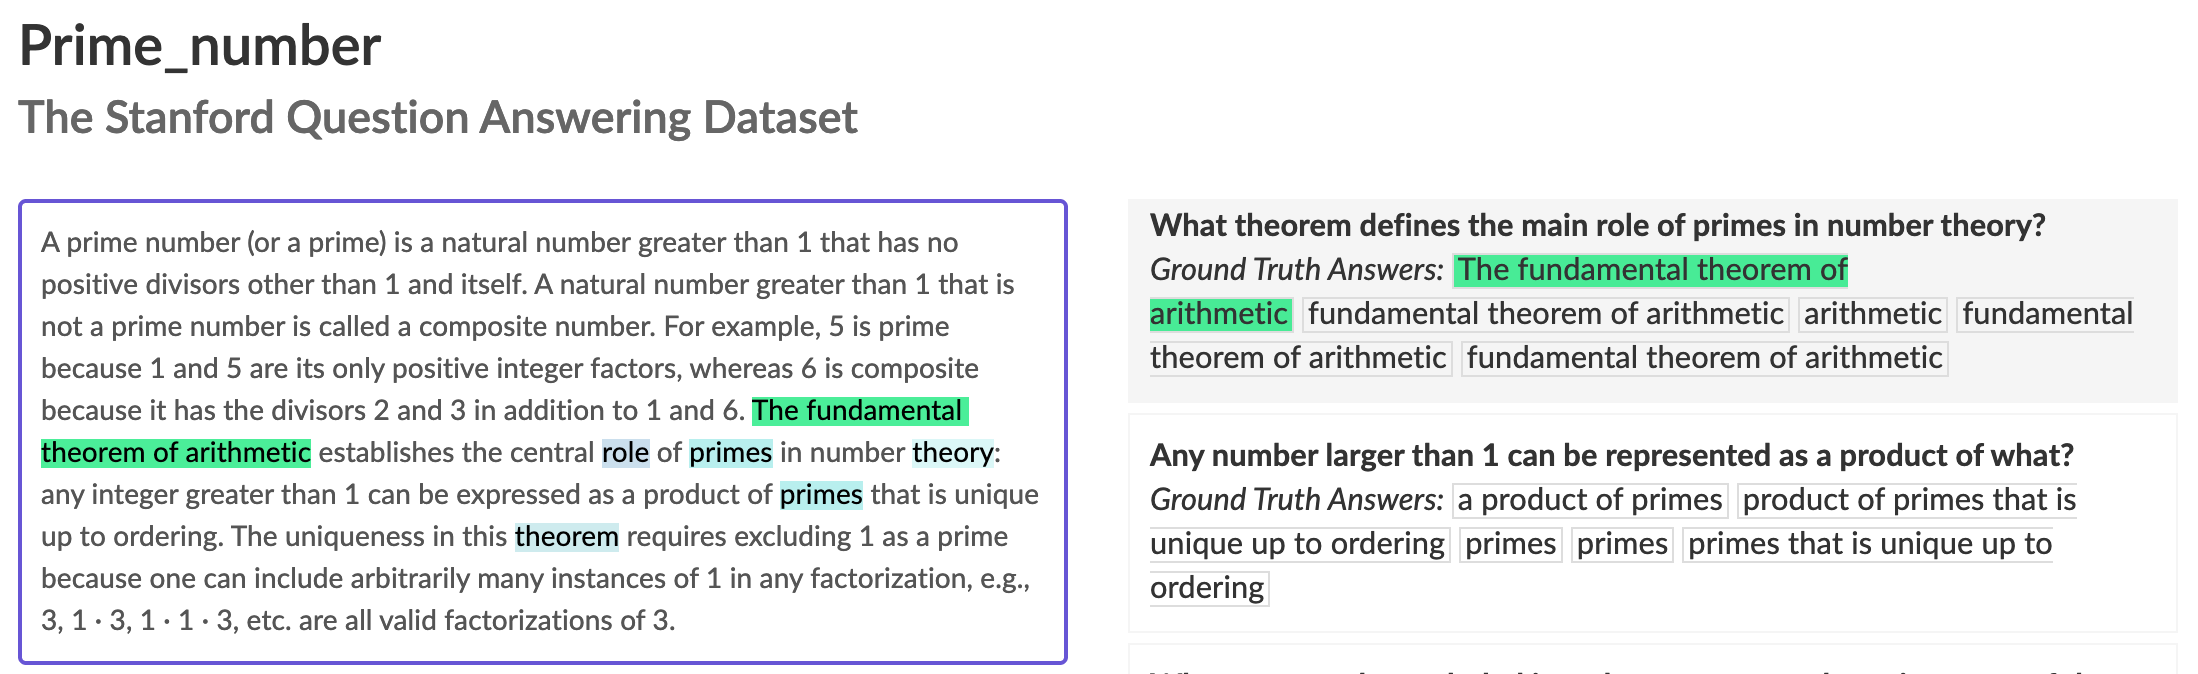
\includegraphics[width=0.95\textwidth]{figures/squad_example.png}
                \label{fig:-squad-example}
            \end{figure}
            

    \section{Theoretical Part}
    \label{sec:theoretical-part}

    % Theoretical part: literature overview: which models from the literature are suitable for this problem given your data and why? which algorithms can be used to train them? how these models are related to your hypothesis? present an overview of your approach: what steps are executed in the learning pipeline? which hyperparameters of the learning algorithm are available and how they can influence the results? You must show that you applied methods considered during the semester to the selected problem. Feel free to include any figures or tables helping to describe your method and compare it with others. If you use information from other sources, please cite it properly.
        Placeholder

    \section{Implementation}
    \label{sec:implementation}


    % Implementation: how did you implement your approach? which tools were used? show interesting snippets or present your algorithms.

        Placeholder

    \section{Evaluation}
    \label{sec:evaluation}

    % Evaluation: present and visualize results of your evaluation, explain what do your results mean, why was your approach successful, why not? compare it to some baseline either implemented yourself or from the literature, blogs, Kaggle, etc.
        Placeholder

    \section{Conclusion}
    \label{sec:conclusion}
    % Conclusions: how can you evaluate the results of your work? what would you recommend for future steps?

        Placeholder

    \section{Supplementary Materials}
    \label{sec:supplementary-materials}

    % Supplementary materials: The report must be submitted as an archive comprising all code and artifacts (data, custom python modules, images, videos, etc.) required for its correct representation, evaluation, and exemplification of your work. If data is too large for a submission, please provide a link where this data can be downloaded from.

    \pagebreak

    \bibliography{references.bib}
    \bibliographystyle{ieeetr}
    % \printbibliography

\end{document}
